% Revised manuscript. Numerical inputs are generated from verified per-seed results.
\RequirePackage[T1]{fontenc}
\documentclass[conference,a4paper]{IEEEtran}
\usepackage{amsmath,amssymb,booktabs,graphicx,cite,url}
\usepackage[hidelinks]{hyperref}
\graphicspath{{figures/revision/}}
\newcommand{\MainClosed}{6.70}
\newcommand{\MainDegraded}{97.53}
\newcommand{\MainQualified}{6.61}
\newcommand{\MainForced}{90.08}
\newcommand{\MainForcedLo}{89.20}
\newcommand{\MainForcedHi}{90.97}
\newcommand{\MainPayloadLoss}{92.24}
\newcommand{\MainNoAttack}{97.53}
\newcommand{\MainQualifiedDelta}{-0.09}
\newcommand{\MainQualifiedDeltaLo}{-0.11}
\newcommand{\MainQualifiedDeltaHi}{-0.07}

\newcommand{\LearnUtilityDelta}{0.0011}
\newcommand{\LearnUtilityDeltaLo}{0.0002}
\newcommand{\LearnUtilityDeltaHi}{0.0020}
\newcommand{\LearnQualifiedDelta}{0.10}
\newcommand{\LearnQualifiedDeltaLo}{0.01}
\newcommand{\LearnQualifiedDeltaHi}{0.20}
\newcommand{\LearnPayloadDelta}{1.71}
\newcommand{\LearnPayloadDeltaLo}{1.55}
\newcommand{\LearnPayloadDeltaHi}{1.85}
\newcommand{\LearnISRDelta}{-2.77}
\newcommand{\LearnISRDeltaLo}{-2.97}
\newcommand{\LearnISRDeltaHi}{-2.59}
\newcommand{\LearnCommandDelta}{0.13}
\newcommand{\LearnCommandDeltaLo}{0.04}
\newcommand{\LearnCommandDeltaHi}{0.23}
\newcommand{\LearnLogisticsDelta}{0.25}
\newcommand{\LearnLogisticsDeltaLo}{0.15}
\newcommand{\LearnLogisticsDeltaHi}{0.36}
\newcommand{\LearnPayloadGreedy}{1.99}
\newcommand{\LearnPayloadMulti}{3.69}
\newcommand{\LearnISRLoss}{2.77}
\newcommand{\LearnShortDelta}{-0.0047}
\newcommand{\LearnLongDelta}{-0.0036}

\newcommand{\StockLowClosed}{6.97}
\newcommand{\StockLowClosedLo}{6.24}
\newcommand{\StockLowClosedHi}{7.59}
\newcommand{\StockMidClosed}{31.65}
\newcommand{\StockMidClosedLo}{29.84}
\newcommand{\StockMidClosedHi}{33.34}
\newcommand{\StockFullClosed}{97.54}
\newcommand{\StockFullClosedLo}{97.34}
\newcommand{\StockFullClosedHi}{97.72}
\newcommand{\DurationHourForced}{0.06}
\newcommand{\DurationHourForcedLo}{0.00}
\newcommand{\DurationHourForcedHi}{0.17}
\newcommand{\DurationSixForced}{17.62}
\newcommand{\DurationSixForcedLo}{17.07}
\newcommand{\DurationSixForcedHi}{18.16}
\newcommand{\DurationDayForced}{89.85}
\newcommand{\DurationDayForcedLo}{89.23}
\newcommand{\DurationDayForcedHi}{90.51}
\newcommand{\AuthLowClosed}{8.53}
\newcommand{\AuthHighClosed}{3.27}
\newcommand{\AuthClosedLoss}{5.26}
\newcommand{\AuthClosedLossLo}{4.34}
\newcommand{\AuthClosedLossHi}{6.07}
\newcommand{\CorrelatedBaseForced}{2.96}
\newcommand{\CorrelatedBaseForcedLo}{1.57}
\newcommand{\CorrelatedBaseForcedHi}{4.39}
\newcommand{\CorrelatedExcess}{86.89}
\newcommand{\CorrelatedExcessLo}{85.57}
\newcommand{\CorrelatedExcessHi}{88.21}
\newcommand{\ShapeForced}{83.47}
\newcommand{\ShapeForcedLo}{82.67}
\newcommand{\ShapeForcedHi}{84.34}
\newcommand{\CutThreeForced}{90.17}
\newcommand{\CutThreeForcedLo}{89.47}
\newcommand{\CutThreeForcedHi}{90.88}
\newcommand{\CutFourForced}{87.47}
\newcommand{\CutFourForcedLo}{86.40}
\newcommand{\CutFourForcedHi}{88.71}
\newcommand{\OnlineRelease}{35.50}
\newcommand{\OnlineReleaseLo}{31.67}
\newcommand{\OnlineReleaseHi}{39.56}
\newcommand{\OnlinePersistent}{89.69}
\newcommand{\OnlinePersistentLo}{89.04}
\newcommand{\OnlinePersistentHi}{90.22}
\newcommand{\OnlinePersistenceGain}{54.19}
\newcommand{\OnlinePersistenceGainLo}{49.72}
\newcommand{\OnlinePersistenceGainHi}{58.08}
\newcommand{\FallbackOnline}{5.03}
\newcommand{\FallbackOnlineLo}{4.47}
\newcommand{\FallbackOnlineHi}{5.60}
\newcommand{\FallbackPreplaced}{97.54}
\newcommand{\FallbackPreplacedLo}{97.35}
\newcommand{\FallbackPreplacedHi}{97.72}
\newcommand{\FallbackTransport}{0.064}
\newcommand{\FallbackTransportLo}{0.042}
\newcommand{\FallbackTransportHi}{0.085}
\newcommand{\FallbackServiceGain}{92.51}
\newcommand{\FallbackServiceGainLo}{91.91}
\newcommand{\FallbackServiceGainHi}{93.08}
\newcommand{\FallbackQualifiedGain}{1.90}
\newcommand{\FallbackQualifiedGainLo}{1.15}
\newcommand{\FallbackQualifiedGainHi}{2.62}

\begin{document}
\title{Fail-Closed or Fail-Degraded? A Simulation Study of Forced Assurance Loss in Contested Multi-Hop QKD Networks}
\author{
\IEEEauthorblockN{Lakshya Jain\IEEEauthorrefmark{1}, Siddhi Arora\IEEEauthorrefmark{2}, Divya Mishra\IEEEauthorrefmark{3}}
\IEEEauthorblockA{\IEEEauthorrefmark{1}\textit{Maharaja Agrasen Institute of Technology}, Delhi, India, 10jainlakshya@gmail.com\\
\IEEEauthorrefmark{2}\textit{Noida Institute of Engineering and Technology}, Greater Noida, India, Sid.arora1701@gmail.com\\
\IEEEauthorrefmark{3}\textit{G.L. Bajaj Institute of Technology and Management}, Greater Noida, India, divya\_rbl2@yahoo.com}}
\maketitle

\begin{abstract}
Stopping quantum key generation need not immediately exhaust a trusted-relay network's stored keys. We study how finite reserves, interruption duration and fallback policy jointly determine timely key service and assurance loss. Generation, transport and online key-establishment failures are separated, with paired policy comparisons within each condition. A 360-run, five-topology grid includes 24-hour generation cuts with only 2\% of usable capacity initially filled. In the eight-node formation, fail-closed service is \MainClosed\%, compared with \MainDegraded\% under fallback; compliant fallback service is only \MainQualified\%. The fraction of offered requests entitled to information-theoretically secure (ITS) key delivery but served below it is \MainForced\% (95\% interval \MainForcedLo--\MainForcedHi\%). With full starting reserves, the same cut produces no observed forced loss in the 24-hour cohort. An interpretable controller trained across several conditions raises mean count-based utility by \LearnUtilityDelta{} on a held-out benchmark, yet increases associated below-ITS payload exposure by \LearnPayloadDelta{} percentage points while respecting every class exception cap. The results characterize modeled key service and contractual exposure, rather than payload throughput or field-validated security.
\end{abstract}
\begin{IEEEkeywords}
Quantum key distribution, trusted relays, key management, post-quantum cryptography, assurance metrics, constrained policy search.
\end{IEEEkeywords}

\section{Introduction}
Quantum key distribution (QKD) supply interruptions can be handled by waiting, blocking or computational fallback. ITU-T Y.3803 permits policy-controlled symmetric relay substitution and records the method~\cite{itu}; Tysowski \emph{et al.} describe fallback and blocking~\cite{tysowski}, and Spooren \emph{et al.} implement layered failure timers~\cite{spooren}. We examine how these choices interact with usable stored key.

A relay formation may mix command-key requests, an expensive one-time-pad (OTP) class and logistics traffic. We distinguish successful key service from satisfaction of its assurance requirement, and loss of replenishment from loss of accepted stored key.

We evaluate finite reserves, interruption duration, relative link-suppression budgets and learned grade allocation under class-specific exception permissions. Timely and floor-compliant service share an arrival denominator; entitlement to information-theoretically secure (ITS) keys, payload and class-importance metrics expose different losses. A cumulative cut-budget inequality and exact fixtures delimit feasible service. The learning study compares a compact controller with a greedy policy under the same monitor.

\section{Related Work}
Adaptive graded key delivery already appears in QuLore~\cite{qulore}, and Q-learning has been applied to resource-aware trusted-relay routing~\cite{hao}. Our learned action is a requested assurance grade. Routing uses the explicitly defined implementation below; the study does not compare against reimplemented published routing algorithms.

Opportunistic QKD studies single-link reservoirs and correlated depletion/recovery~\cite{opportunistic}; QuIKS combines end-to-end buffering, reactive control and device traces~\cite{quiks}; Zhu studies finite buffers, fallback fractions and class-sensitive output~\cite{zhu}. Building on these, we jointly evaluate targeted generation interruptions, relative link costs, paired excess entitlement loss and learned class-exception allocation.

Established runtime filtering~\cite{shield} motivates our deterministic prefix-count exception monitor, whose contract is specified below.

\section{Model and Assurance Accounting}\label{sec:model}
\subsection{Stored key and failure surfaces}
A trusted-relay graph has one shared key store per undirected link. Relaying a session key debits every traversed link once. For link $e$, stored stock obeys
\begin{equation}\label{eq:stock}
B_e(t)=B_e(0)+G_e(t)-C_e(t)-O_e(t)-P_e(t),
\end{equation}
where $G_e$ is gross incoming distilled-key supply before buffer overflow, $C_e$ useful relay consumption, $O_e$ overflow discard, and $P_e$ intentional working-key purge. Usable stock is $U_e=(B_e-b_{\min})_+$. Admission checks every hop before any debit; partial relay transactions and in-flight failures are outside this abstraction.

Stored keys are retained while synchronized, unexpired and uncompromised. The purge alternative discards spendable stock when generation fails but preserves the protected reserve. These alternatives reflect the generation/storage distinction~\cite{itu} and implementation-dependent shutdown or synchronization policies~\cite{tysowski}. The reserve is an unavailable inventory floor; periodic QKD post-processing does not debit it in this model. Its presence therefore does not establish authentication continuity during an outage.

Generation suppression leaves classical relay transport available. A transport-disconnected request cannot be served, even with pre-positioned key material. An isolated online key-establishment failure is a third surface: it can prevent a key-encapsulation-mechanism (KEM) fallback without blocking a valid pre-positioned symmetric key. These surfaces are modeled separately.

Nominal generation is a parameterized input. For quantum bit error rate (QBER) $x$, nominal $x_0=0.03$ and reconciliation factor $f=1.16$, we use the reduced response
\begin{equation}\label{eq:rate}
\frac{R_e(x)}{R_{e,0}}=\left[\frac{\max\{0,1-(1+f)H_2(x)\}}{1-(1+f)H_2(x_0)}\right]^{\gamma}
\end{equation}
below $x_{\mathrm{abort}}$, and zero at or above it; $H_2$ is binary entropy in bits and the ratio is capped at one. The engineering threshold is 0.075, with 0.11 as a sensitivity. The entropy numerator can become zero before a selected abort threshold, so the latter alone does not set the zero-rate boundary. The exponents 1 and 3.4 are illustrative response shapes, not a cross-modality calibration or a finite-key security proof.

\subsection{Grades, requests and debits}
The policy order is G1, G2, G3, G4. G1 requires payload-length OTP key; G2 a 256-bit QKD-delivered symmetric key; G3 128 QKD bits as a hybrid ingredient; and G4 no quantum key. G2 classifies information-theoretic key delivery with computational payload encryption. The ordering specifies contracts, not universal cryptographic strength or hybrid-combiner security.

For a nonzero quantum-key demand $D_g$, the per-hop debit is
\begin{equation}\label{eq:debit}
q_g=D_g+240+127n_{\mathrm{auth}}\quad\text{bits}.
\end{equation}
The metadata allocation is an explicit choice within the key-file abstraction of Y.3803~\cite{itu}. The tag size is motivated by Walenta \emph{et al.}~\cite{walenta}; reusable-hash authentication charges are discussed by Fung \emph{et al.}~\cite{fung}. These sources do not establish a universal number of authenticated messages per relayed request. We use $n_{\mathrm{auth}}=7$ as a conservative relay-overhead setting relative to the optimistic value 2, and also evaluate 40. The corresponding G2 debits are 1385, 750 and 5576 bits per hop. This is a simplified cost model, not protocol-level calibration.

Command-and-control (C2), intelligence/surveillance/reconnaissance (ISR), and logistics (LOG) requests have payloads 2048, 144000 and 320000 bits; floors G2, G1 and G3; deadlines 5, 30 and 120 seconds; and strict scheduling priorities in that order. Independent Poisson arrival rates are 0.05, 0.002 and 0.03 per second in the reduced-load case. These are declared workload scenarios. The required mean key debit is 397.218 bits/s across a cut traversed once per request, compared with 480 bits/s for two nominal 240-bit/s branches. This is a nominal capacity check, not a queue-stability proof. ISR arrival-rate factors 0.03, 0.1 and 1 relative to 0.02/s separate lighter load from overload.

\subsection{Common-denominator outcomes}\label{sec:metrics}
For all $N$ requests arriving in a fixed observation window, let $S$ receive key service within their deadlines and $D\subseteq S$ receive a grade below their class floor. Define
\begin{equation}\label{eq:metrics}
A=\frac{|S|}{N},\qquad Q=\frac{|S\setminus D|}{N},\qquad L=\frac{|D|}{N}.
\end{equation}
Thus $A=Q+L$; blocking is $1-A$. This identity makes fallback's service advantage distinguishable from floor compliance.

Let $E$ be requests entitled to G1 or G2, and $D_{\mathrm{ITS}}\subseteq E\cap S$ those served at G3 or G4. Offered-request forced assurance loss is $F=|D_{\mathrm{ITS}}|/|E|$. ITS-delivered, below-ITS-delivered and blocked fractions sum to one on this entitled-arrival cohort. The accompanying tables retain $F_{\mid S}=|D_{\mathrm{ITS}}|/|E\cap S|$ separately. LOG is excluded from the ITS-entitled denominator.

For associated payload size $b_s$, define $F_B=\sum_{s\in D_{\mathrm{ITS}}}b_s/\sum_{s\in E}b_s$; $L_B$ similarly weights below-floor service over all arrivals. These are exposure proxies, not observed compromise or calibrated harm. Class-importance vectors $(1,1,1)$, $(5,2,1)$ and $(10,3,1)$ provide another transparent reweighting. Attack-attributable change is a paired attacked-minus-unattacked difference under the same exogenous environment; no zero baseline is assumed.

For example, an ISR request served at G2 violates its G1 floor and contributes to $L$, while retaining the modeled ITS key-delivery entitlement and hence not contributing to $F$. An allowed exception still counts as a floor violation: permission to accept a weaker grade does not rewrite the original requirement. A fraction with an empty denominator is undefined, recorded as null alongside its counts, and is never interpreted as zero loss.

\subsection{A finite cut-budget check}\label{sec:bound}
For an edge cut $\delta(W)$, $W\subset V$, every compliant relay between separated endpoints must consume key on a crossing edge. Let $\mathcal C_T$ contain these compliant requests completed by time $T$, and $q_s$ be their minimum per-hop debit. Then
\begin{equation}\label{eq:cut}
\sum_{s\in\mathcal C_T}q_s
\leq\sum_{e\in\delta(W)}\left[U_e(0)+G_e(T)\right].
\end{equation}
Discard, competing traffic and repeated cut crossings only tighten this upper bound. Each completed compliant request contributes at least $q_s$ to consumption summed over the cut. Equation~\ref{eq:stock} and nonnegative final usable stock then bound that sum by initial usable stock plus generation; dropping nonnegative discard and competing consumption yields~\eqref{eq:cut}. This is a necessary resource condition, not a sufficient scheduling condition. It does not account for whether key reaches the right path before a deadline. A generation cut removes replenishment, not the initial term.

The pooled bound need not be attainable. With three disjoint two-hop branches, 1900 spendable bits per edge and a 750-bit debit, it permits seven requests, but the simulator serves only six: each branch retains an unusable 400-bit fragment. Four 749-bit stores permit three requests under the pooled relaxation and none in the actual graph. Exact divisible-stock and purge cases also pass. These fixtures check implementation and the bound's scope.

\section{Policies and Experimental Protocol}\label{sec:protocol}
\subsection{Compared control policies}
Fail closed waits for the authorized floor and blocks at deadline. Unrestricted fallback attempts progressively weaker grades when that floor cannot be met. Our shortest-path baseline chooses the first transport-usable minimum-hop candidate. The key-aware implementation minimizes bottleneck estimated refill time plus a 0.5-second penalty per hop. Candidate enumeration is limited to four simple paths within two extra hops of the shortest. The comparison concerns these implementations.

The learned controller uses 18 states: three classes, three floor-feasibility categories, and two deadline-urgency categories. Feasibility distinguishes affordable now, refill estimated within the remaining deadline, and neither; urgency means at most 20\% of the deadline remains. Estimated refill uses current rates and ignores future competing arrivals. The five proposed actions are the class floor, strongest affordable fallback, defer, G4 and G2.

All learned and budget-greedy actions pass through the same monitor. If $N_c(t)$ class-$c$ requests have arrived and $V_c(t)$ below-floor services have been committed, a proposed exception is permitted only when
\begin{equation}\label{eq:budget}
V_c(t)+1\leq\lfloor\epsilon_cN_c(t)\rfloor,
\end{equation}
with $(\epsilon_{\mathrm{C2}},\epsilon_{\mathrm{ISR}},\epsilon_{\mathrm{LOG}})=(0,0.1,0.1)$. Failed attempts spend no allowance. Since arrivals only increase the right-hand side and every committed exception is checked before use, induction gives the prefix bound. Completed exceptions are a subset of committed exceptions. This is an arrival-count permission guarantee within the simulator, not a learned cryptographic guarantee. Strict-floor and greedy policies are explicit baselines.

Categorical cross-entropy policy search~\cite{cem} uses ten unique tables per generation, four generations and two optimizer restarts. Every generation includes the strict, greedy and incumbent tables. Short-nominal training uses six-hour rollouts; full-nominal uses 24 hours; full-robust uses a mean over nominal, generation-cut and correlated low-rate conditions. Each candidate receives six rollouts. Validation selects between the two training-selected finalists on three conditions and four separate seeds. Final testing uses twelve previously unused seeds over seven fixed conditions, including unseen topologies. The objective $J=A-0.75L=Q+0.25L$ assigns one-quarter value to below-floor service. Tables, histories, objective, validation rule and test plan are frozen before final testing; optimality is not established.

Per-state action probabilities start uniformly at 0.2. The top three training candidates form the elite set, with a 0.5 pseudocount per action before normalization for the next generation. Optimizer seeds 7000 and 7001 are paired across regimes. Simulator seeds 1000--1005, 2000--2003 and 5000--5011 are reserved for training, validation and testing, respectively. Robust training assigns two of its six rollouts to each condition; it optimizes their mean rather than the worst case. Repeated candidate tables reuse identical cached rollouts, which do not add independent evidence. The 18-cell observation records class, floor feasibility and deadline urgency, omitting full inventory and queue state; the controller does not observe the full network state, and the search establishes no policy optimality.

\subsection{Scenarios, uncertainty and verification}
The graph families are an eight-node, nine-link formation; an eight-node ring; a $3\times3$ grid; and three or four parallel three-hop branches. The latter have $(8,9)$ and $(10,12)$ nodes/edges. Individual formation terminals are leaves, with cut size one; isolating all formation terminals requires two edges. The other source-terminal cut sizes are two, two, three and four. These different notions of cut are not conflated.

Formation rates are 200--400 bits/s on eight free-space links and 300 kbits/s on one fiber; the other graphs use 240-bit/s links. Capacities, threshold and reserve are selected legacy QKDNetSim example parameters~\cite{qkdnetsim}: 52428800, 11324620 and 1048576 bits. Capacity is 50 Mibit, not a measured hardware specification. Our overflow model clamps continuous stock and discards excess; it is not byte-for-byte equivalence to a discrete block buffer. Initial spendable fractions are 0.02, 0.1 and 1; the main stressed initial stock is 1027604.48 usable bits per edge.

Link-suppression cost is one for free-space links and ten for fiber, with ratios one and one hundred as sensitivities. These are relative scenario weights, not measured adversary expenditure. A weighted source-to-all-terminals cut is a structural reference, not an optimal finite-horizon attack. Main generation attacks add $\Delta x=0.05$ to selected links, taking their nominal QBER from 0.03 to 0.08, above the 0.075 engineering abort threshold. Independent free-space generation and all-link transport failures use declared mean up/down times of 3600/120 seconds. The correlated-generation sensitivity gives all free-space generators a common 900/600-second up/down process. Policy comparisons within each condition share exogenous draws that are independent of policy and attack choices.

Simulation uses one-second steps and a 24-hour arrival window without a steady-state claim. Pending requests are followed to their deadlines; an interruption scheduled to end at 24 hours can release before the last completion. Equation~\ref{eq:cut} uses the completion horizon for such a cohort. Twelve seeds support the main grid, eight the sensitivity and fallback comparisons, and six the threshold sweeps. Percentages are means of seedwise proportions. Intervals are marginal 95\% percentile bootstrap intervals over independent seeds, with 20000 resamples, conditional on the parameters and, for learning, the selected table.

Within a tick, outages and attack status are updated first, followed by one tick of generation, Poisson arrival counts, and service attempts in class-priority/FIFO order. Pending requests retry on later ticks. G3/G4 online establishment adds a selected 0.35-second completion delay; G1/G2 and ideal pre-positioned fallback add none. The predicted completion must meet the deadline before any debit, and equality at the deadline is accepted. These are atomic admission transactions, not simulated KEM packet exchanges. All revision cohorts start at time zero without a discarded warmup; the follow-up admits no new requests. Conservation compares counters over the same event horizon, rather than mixing arrival-cohort consumption with generation measured only before the follow-up.

\subsection{Verification scope}
Verification checks conservation, reserve and deadline invariants, exact resource fixtures, matched exogenous traces and prefix budgets. The historical four-check literature comparison is retained in the artifact with explicit limits: V1 is stored-volume/rate arithmetic, and V4 is a coarse capacity plausibility calculation. V2 and V3 are the two mismatches, involving inferred global-key size and application-tunnel consumption versus a per-hop charge, respectively. They do not uniquely calibrate the authentication-message count. Neither V1 nor V4 is an independent reproduction of network policy behavior. Published sources motivate parameter choices; implementation checks do not validate network predictions against hardware or establish cryptographic security.

\section{Results}\label{sec:results}
\subsection{Availability is not compliant service}
At the main low-reserve setting, suppressing the weighted generation cut leaves formation fail-closed service at \MainClosed\%, compared with \MainNoAttack\% without attack. Fallback serves \MainDegraded\% of arrivals, but only \MainQualified\% meet their original floor. Its compliant-service difference from fail closed is \MainQualifiedDelta\ percentage points, with interval $[\MainQualifiedDeltaLo,\MainQualifiedDeltaHi]$. The large availability difference therefore cannot be interpreted as preserved authorized protection.

\begin{figure}[t]
\centering
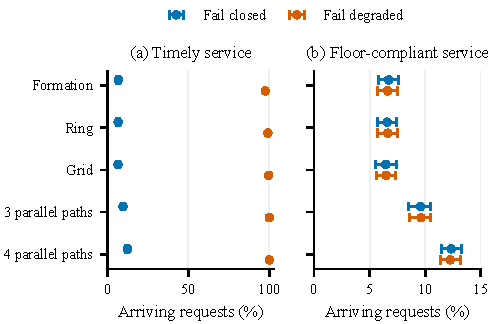
\includegraphics[width=\columnwidth]{fig1_comparable_service.pdf}
\caption{Timely and floor-compliant key service under full generation-cut suppression, 24-hour arrival cohorts and 2\% initial usable stock. Bars are 95\% seed-bootstrap intervals ($n=12$). The horizontal scales differ.}
\label{fig:service}
\end{figure}

\begin{table}[t]
\caption{Formation class outcomes under the two-edge generation cut. Entries are percent of class arrivals; 95\% intervals appear below the means, from 12 seeds.}
\label{tab:classes}
\centering\footnotesize
\setlength{\tabcolsep}{3pt}
\begin{tabular}{@{}lccc@{}}
\toprule
Class & Closed $Q$ & Fallback $A$ & Fallback $Q$\\
\midrule
C2 & \shortstack{6.67\\(5.70, 7.61)} & \shortstack{96.72\\(96.52, 96.89)} & \shortstack{6.65\\(5.68, 7.59)}\\[3pt]
ISR & \shortstack{5.67\\(5.41, 5.97)} & \shortstack{97.50\\(96.66, 98.32)} & \shortstack{5.67\\(5.41, 5.97)}\\[3pt]
LOG & \shortstack{6.83\\(5.91, 7.67)} & \shortstack{98.88\\(98.74, 99.01)} & \shortstack{6.60\\(5.73, 7.41)}\\[3pt]
\bottomrule
\end{tabular}

\end{table}

Figure~\ref{fig:service} shows the same distinction across all five graphs. Table~\ref{tab:classes} prevents an aggregate score from hiding a class's admission failure. Formation forced loss is \MainForced\% of offered ITS-entitled requests, whereas below-floor payload exposure $L_B$ is \MainPayloadLoss\% of all associated payload bits. The different values reflect different denominators and requirements.

\subsection{Reserve and operating-envelope dependence}\label{sec:sensitivity}
The eight-seed stock sweep changes the interpretation substantially. Under the same formation cut, fail-closed service is \StockLowClosed\%, \StockMidClosed\% and \StockFullClosed\% at 2\%, 10\% and 100\% initial usable fill. Full-stock runs show no forced loss and the two modes have equal service. At 2\% fill, six-hour suppression produces $F=\DurationSixForced\%$ $[\DurationSixForcedLo,\DurationSixForcedHi]$, compared with \DurationDayForced\% for 24 hours. Figure~\ref{fig:reserve} shows why a cut size without a stock level and observation window is insufficient.

Table~\ref{tab:load} isolates offered ISR load while holding the formation cut, initial stock and other assumptions fixed. Relative to the original 0.02/s ISR rate, the 0.03 factor yields a paired availability gap of 85.42 points, compared with 94.72 points at the original rate. Fallback availability remains approximately 97.5\%, but its compliant service tracks fail-closed service. Reduced load narrows rather than eliminates the gap in this low-stock cohort; the full-stock comparison separately shows that this outcome is not universal. The eight-seed sensitivity estimates are distinct from the twelve-seed main estimates.

\begin{table}[t]
\caption{ISR-load sensitivity under the formation generation cut and 2\% usable fill. Service columns are seed-mean percentages; $\Delta A$ is fallback minus closed, with its paired 95\% interval below ($n=8$).}
\label{tab:load}
\centering\footnotesize
\setlength{\tabcolsep}{3pt}
\begin{tabular}{@{}lccc@{}}
\toprule
ISR factor & Closed $A$ & Fallback $Q$ & $\Delta A$ (pp)\\
\midrule
0.03 & 12.11 & 12.06 & \shortstack{85.42\\(83.84, 86.71)}\\[3pt]
0.1 & 6.97 & 6.87 & \shortstack{90.56\\(90.04, 91.10)}\\[3pt]
1 & 2.75 & 2.27 & \shortstack{94.72\\(94.47, 95.03)}\\[3pt]
\bottomrule
\end{tabular}

\end{table}

\begin{figure}[t]
\centering
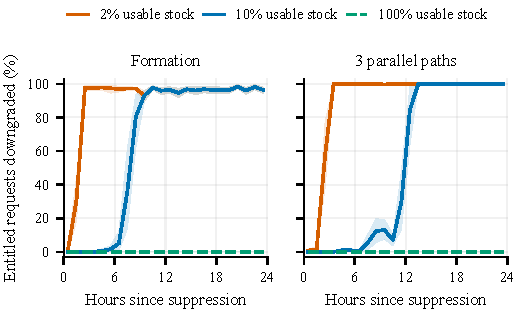
\includegraphics[width=\columnwidth]{fig2_reserve_horizon.pdf}
\caption{Hourly entitled-arrival loss under a held generation cut, with 2\%, 10\% and 100\% initial usable fill. Lines and pointwise 95\% bands use eight seeds. These are hourly cohorts, not a cumulative failure probability.}
\label{fig:reserve}
\end{figure}

Accounting remains consequential: raising $n_{\mathrm{auth}}$ from 2 to 40 reduces closed service from \AuthLowClosed\% to \AuthHighClosed\%, a paired loss of \AuthClosedLoss{} points $[\AuthClosedLossLo,\AuthClosedLossHi]$. Common-cause generation outages already produce unattacked $F=\CorrelatedBaseForced\%$ $[\CorrelatedBaseForcedLo,\CorrelatedBaseForcedHi]$; the paired attack excess is \CorrelatedExcess{} points $[\CorrelatedExcessLo,\CorrelatedExcessHi]$. Observed loss is therefore not automatically attack-attributable.

With $\gamma=1$, no environmental outages and increment $\Delta x=0.045$, full three- and four-path cuts produce $F=\CutThreeForced\%$ $[\CutThreeForcedLo,\CutThreeForcedHi]$ and \CutFourForced\% $[\CutFourForcedLo,\CutFourForcedHi]$; at increment 0.03 both are zero. At $\Delta x=0.04$, absolute QBER is 0.07, below the 0.075 engineering abort. The three-path case then gives $F=0$ for $\gamma=1$ and \ShapeForced\% $[\ShapeForcedLo,\ShapeForcedHi]$ for the illustrative $\gamma=3.4$ response. Slow positive generation can force loss before abort; an engineering threshold and a minimum cut do not define a universal finite-horizon forcing rule.

\subsection{Target persistence and attack cost}\label{sec:persistence}
Table~\ref{tab:cost} compares three selectors at relative budget two. Static ranking uses initial edge betweenness divided by link cost. Offline residual ranking recomputes source-to-still-reachable-terminal betweenness per cost after each structural removal; it is distinct from the online route-feedback controller below. The cut reference minimizes total weight for isolating all terminals. Raising fiber cost from one to ten or one hundred excludes fiber from budget-two selections and changes residual-ranking loss substantially, while these static and cut outcomes remain unchanged. The table therefore supports a cost- and method-conditioned result, not a claim that fiber is physically unattackable or that any selector optimizes finite-horizon loss.

\begin{table}[t]
\caption{Offered-entitlement loss $F$ (\%) at relative budget two. Free-space cost is one; means and 95\% seed intervals use eight formation runs per cell. Residual denotes the offline residual ranking.}
\label{tab:cost}
\centering\footnotesize
\setlength{\tabcolsep}{2.5pt}
\begin{tabular}{@{}lccc@{}}
\toprule
Fiber cost & Static & Residual & Cut\\
\midrule
1 & \shortstack{58.65\\(58.15, 59.31)} & \shortstack{89.82\\(89.22, 90.46)} & \shortstack{89.85\\(89.23, 90.51)}\\[3pt]
10 & \shortstack{58.65\\(58.15, 59.31)} & \shortstack{10.13\\(8.72, 11.52)} & \shortstack{89.85\\(89.23, 90.51)}\\[3pt]
100 & \shortstack{58.65\\(58.15, 59.31)} & \shortstack{10.13\\(8.72, 11.52)} & \shortstack{89.85\\(89.23, 90.51)}\\[3pt]
\bottomrule
\end{tabular}

\end{table}

At tested two-path chain depths $d=2,\ldots,6$, deterministic fixed-centrality prefixes require $d+1$ or $d+2$ removals depending on tie handling, despite connectivity two. At depths two, four and six, we also test an online selector using past committed-route counts and current transport reachability. Every 60 seconds it maximizes uncovered route weight per link cost; unobserved viable paths receive weight 0.01. A six-seed exploratory study releases targets when routes become unusable. A post-hoc diagnostic on six disjoint seeds retains targets to fill unused slots.

Feedback counts successful positive-quantum-key route commitments within the preceding 60-second interval, excludes G4, and resets after each update. The selector observes neither future arrivals nor stored-key inventories.

At depth six and two slots, retaining targets raises excess $F$ from \OnlineRelease\% to \OnlinePersistent\%, a paired increase of \OnlinePersistenceGain{} points $[\OnlinePersistenceGainLo,\OnlinePersistenceGainHi]$. The persistent variant spends 48 relative-cost link-hours and becomes a fixed cover, matching the structural-cut outcomes at depths two, four and six. This identifies persistence/exposure as the intervention, not an intrinsic advantage of adaptivity. Concurrent capacity, realized link-time and distinct links touched are reported separately; retargeting overhead is unmodeled.

\subsection{Learning and the exposure trade-off}\label{sec:learning}
Across the seven fixed test conditions, the multi-condition controller improves mean utility over budget-greedy by $\Delta J=\LearnUtilityDelta$ with interval $[\LearnUtilityDeltaLo,\LearnUtilityDeltaHi]$. Mean compliant service increases \LearnQualifiedDelta{} percentage points. This is a small, objective-dependent gain: associated below-ITS payload exposure rises from \LearnPayloadGreedy\% to \LearnPayloadMulti\%, a paired increase of \LearnPayloadDelta{} points $[\LearnPayloadDeltaLo,\LearnPayloadDeltaHi]$.

\begin{figure}[t]
\centering
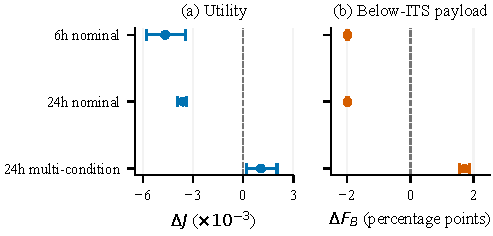
\includegraphics[width=\columnwidth]{fig3_learning_tradeoff.pdf}
\caption{Learned policies relative to budget-greedy. Seven condition means are first averaged within each of 12 held-out seeds; bars are paired 95\% intervals. Higher $J$ is favorable, while higher $F_B$ means more associated entitled payload served below ITS.}
\label{fig:learning}
\end{figure}

The class breakdown explains the aggregate: C2 and LOG compliant service increase \LearnCommandDelta{} and \LearnLogisticsDelta{} points, while ISR compliant service falls \LearnISRLoss{} points. All recorded prefix audits respect the declared class caps. The two additional priority vectors preserve the small positive mean utility difference when reweighting these frozen outcomes. The six-hour and 24-hour nominal training regimes instead change mean utility by \LearnShortDelta{} and \LearnLongDelta{} relative to greedy; the latter selects the strict-floor table. Figure~\ref{fig:learning} reports these unfavorable outcomes alongside the multi-condition gain. Count-based scores and class exception caps therefore leave a separate payload-exposure trade-off.

\subsection{Key establishment is not data transport}\label{sec:fallback}
With the generation cut and online key-establishment service unavailable, timely key service is \FallbackOnline\%. Ideal pre-positioned secrets restore \FallbackPreplaced\%, a paired gain of \FallbackServiceGain{} points $[\FallbackServiceGainLo,\FallbackServiceGainHi]$, but compliant service improves only \FallbackQualifiedGain{} points $[\FallbackQualifiedGainLo,\FallbackQualifiedGainHi]$. Under the transport cut both variants serve \FallbackTransport\% of the arrival cohort, entirely after cut release during deadline follow-up. Neither serves through the active cut. This pre-positioned-key comparison assumes sufficient unexpired material; lifetime, refresh and distribution costs are outside the model.

\section{Discussion and Limitations}\label{sec:limits}
The simulator assumes trusted relays, synchronized valid stores, instant state information and atomic debits. It does not model payload transmission, cipher/KEM execution or compromised key material. Finite candidate routes, fixed class payloads and illustrative supply/outage processes limit external validity. Payload and priority weights summarize modeled exposure, not realized harm.

Finite buffers, depletion analysis and runtime shielding have established precedents. The practical question here is their interaction with explicit entitlement, interruption cost and a constrained learned controller. A favorable scalar utility does not waive a class requirement, and a low forced-loss value can result from blocking rather than preserving service. Both outcomes must remain visible. Training-horizon comparisons concern the registered protocols, including their different simulated exposure and state coverage; they do not isolate depletion as the unique cause of a learned-policy difference.

\section{Conclusion}
For finite-reservoir trusted-relay QKD, a generation cut, a key-store policy and a service policy are separate decisions. Starting stock, rate response and target persistence prevent cut size alone from determining finite-horizon assurance loss. Fallback can preserve timely key service while adding little compliant service. A learned allocator can also improve a count-based score within all class caps while increasing entitled-payload exposure. Reporting these outcomes together makes the operational trade-off explicit.

\section*{Reproducibility and Acknowledgement}
The artifact includes fixed configurations, raw per-seed outcomes, source hashes, numerical-table and figure generators, tests, policy-search histories and a validation-selected policy freeze. Historical outputs are preserved separately. The authors used a large language model to assist coding, analysis and drafting; the reported numerical evidence is generated by the accompanying executable experiments.

\begin{thebibliography}{00}
\bibitem{itu} ITU-T, \emph{Quantum key distribution networks---Key management}, Recommendation Y.3803, Dec. 2020.
\bibitem{tysowski} P. K. Tysowski, X. Ling, N. L\"utkenhaus, and M. Mosca, ``The engineering of a scalable multi-site communications system utilizing quantum key distribution (QKD),'' \emph{Quantum Sci. Technol.}, vol. 3, 024001, 2018, doi: 10.1088/2058-9565/aa9a5d.
\bibitem{spooren} P. Spooren, A. Neuhold, S. Ramacher, and T. Huehn, ``PQC-enhanced QKD networks: A layered approach,'' in \emph{Proc. IEEE QCNC}, 2026, doi: 10.1109/QCNC69040.2026.00060.
\bibitem{qulore} A. Sanz \emph{et al.}, ``QuLore: An adaptive security framework to extend quantum-safe communications to real-world networks,'' arXiv:2511.22416v2, 2026.
\bibitem{hao} Y. Hao \emph{et al.}, ``Q-learning for resource-aware and adaptive routing in trusted-relay QKD network,'' \emph{Photonics}, vol. 12, no. 10, 969, 2025, doi: 10.3390/photonics12100969.
\bibitem{opportunistic} S. Chaudhary, P. Munar Vallespir, A. Viladomat Jasso, and J. Noetzel, ``Opportunistic QKD: Exploiting idle capacity of classical WDM systems,'' arXiv:2604.12982v2, 2026.
\bibitem{quiks} Y. Chen \emph{et al.}, ``QuIKS: Near-zero latency key supply with adaptive buffering for resource-efficient quantum key distribution networks,'' arXiv:2604.09144v1, 2026.
\bibitem{zhu} Z. Zhu, ``Techno-economic feasibility analysis of quantum key distribution for power-system communications,'' arXiv:2510.15248v1, 2025.
\bibitem{shield} M. Alshiekh \emph{et al.}, ``Safe reinforcement learning via shielding,'' arXiv:1708.08611v2, 2017.
\bibitem{walenta} N. Walenta \emph{et al.}, ``A fast and versatile QKD system with hardware key distillation and wavelength multiplexing,'' \emph{New J. Phys.}, vol. 16, 013047, 2014, doi: 10.1088/1367-2630/16/1/013047.
\bibitem{fung} C.-H. F. Fung, X. Ma, and H. F. Chau, ``Practical issues in quantum-key-distribution post-processing,'' \emph{Phys. Rev. A}, vol. 81, 012318, 2010, doi: 10.1103/PhysRevA.81.012318.
\bibitem{cem} R. Rubinstein, ``The cross-entropy method for combinatorial and continuous optimization,'' \emph{Methodol. Comput. Appl. Probab.}, vol. 1, pp. 127--190, 1999, doi: 10.1023/A:1010091220143.
\bibitem{qkdnetsim} QKDNetSim, ``SECOQC example and key-buffer implementation,'' \emph{qkdnetsim-v1-old}, commit 394bfed, 2024. [Online]. Available: \url{https://github.com/QKDNetSim/qkdnetsim-v1-old}
\end{thebibliography}
\end{document}
